
% This LaTeX was auto-generated from MATLAB code.
% To make changes, update the MATLAB code and republish this document.

\documentclass{article}
\usepackage{graphicx}
\usepackage{color}

\sloppy
\definecolor{lightgray}{gray}{0.5}
\setlength{\parindent}{0pt}

\begin{document}

    
    \begin{verbatim}
% Put together a list of `n` 2x2 simple geometric transformations
clear
A_lst(:,:,1) = [1 0; 0 1];                           % First matrix
A_lst(:,:,2) = [-1 0; 0 1];                          % Second matrix
A_lst(:,:,3) = [1 0; 0 -1];                          % Third matrix
A_lst(:,:,4) = [cos(pi/2) -sin(pi/2); sin(pi/2) cos(pi/2)]; % Fourth matrix
A_lst(:,:,5) = [1/2 0; 0 1];                         % Fifth matrix
A_lst(:,:,6) = [1 0; 0 1/2];                         % Sixth matrix
A_lst(:,:,7) = [1 0.5; 0 1];                           % Seventh matrix
A_lst(:,:,8) = [1 0; 0.5 1];                           % Eighth matrix

% Define the house
H = [[0;0], [0;1], [1;1.5], [1;1], [1;0], [0;0]];

% Create the first figure
figure(1)

% Plot the house
plot(H(1,:), H(2,:), '-o', 'Color', 'blue', 'MarkerFaceColor', 'red')
title('Original image')

xlim([-2 2])
axis equal

% Get the number of 2x2 matrices
numMatrices = size(A_lst,3);

% Create a second figure
figure(2)
set(gcf, 'Position', [100, 100, 800, 1200]);

transf = {"Scaling by factor of 1", "Reflection about y-axis", "Reflection about x-axis", "Rotation by 90°", "Horizontal Shrink by factor of 1/2", "Vertical shrink by factor of 1/2", "Horizontal shear by 1/2", "Vertical Shear by 1/2"};

for i = 1:numMatrices
    H_transformed = A_lst(:,:,i) * H;
    subplot(ceil(sqrt(numMatrices)), ceil(sqrt(numMatrices)), i); % Create subplots
    plot(H_transformed(1,:), H_transformed(2,:), '-o', 'Color', 'blue', 'MarkerFaceColor', 'red');
    title(['Transformation ' transf(i)], "FontSize", 10);
    xlim([-2 2]);
    ylim([-2 2]);
    axis equal;
end
\end{verbatim}

\includegraphics [width=4in]{transformations_01.eps}

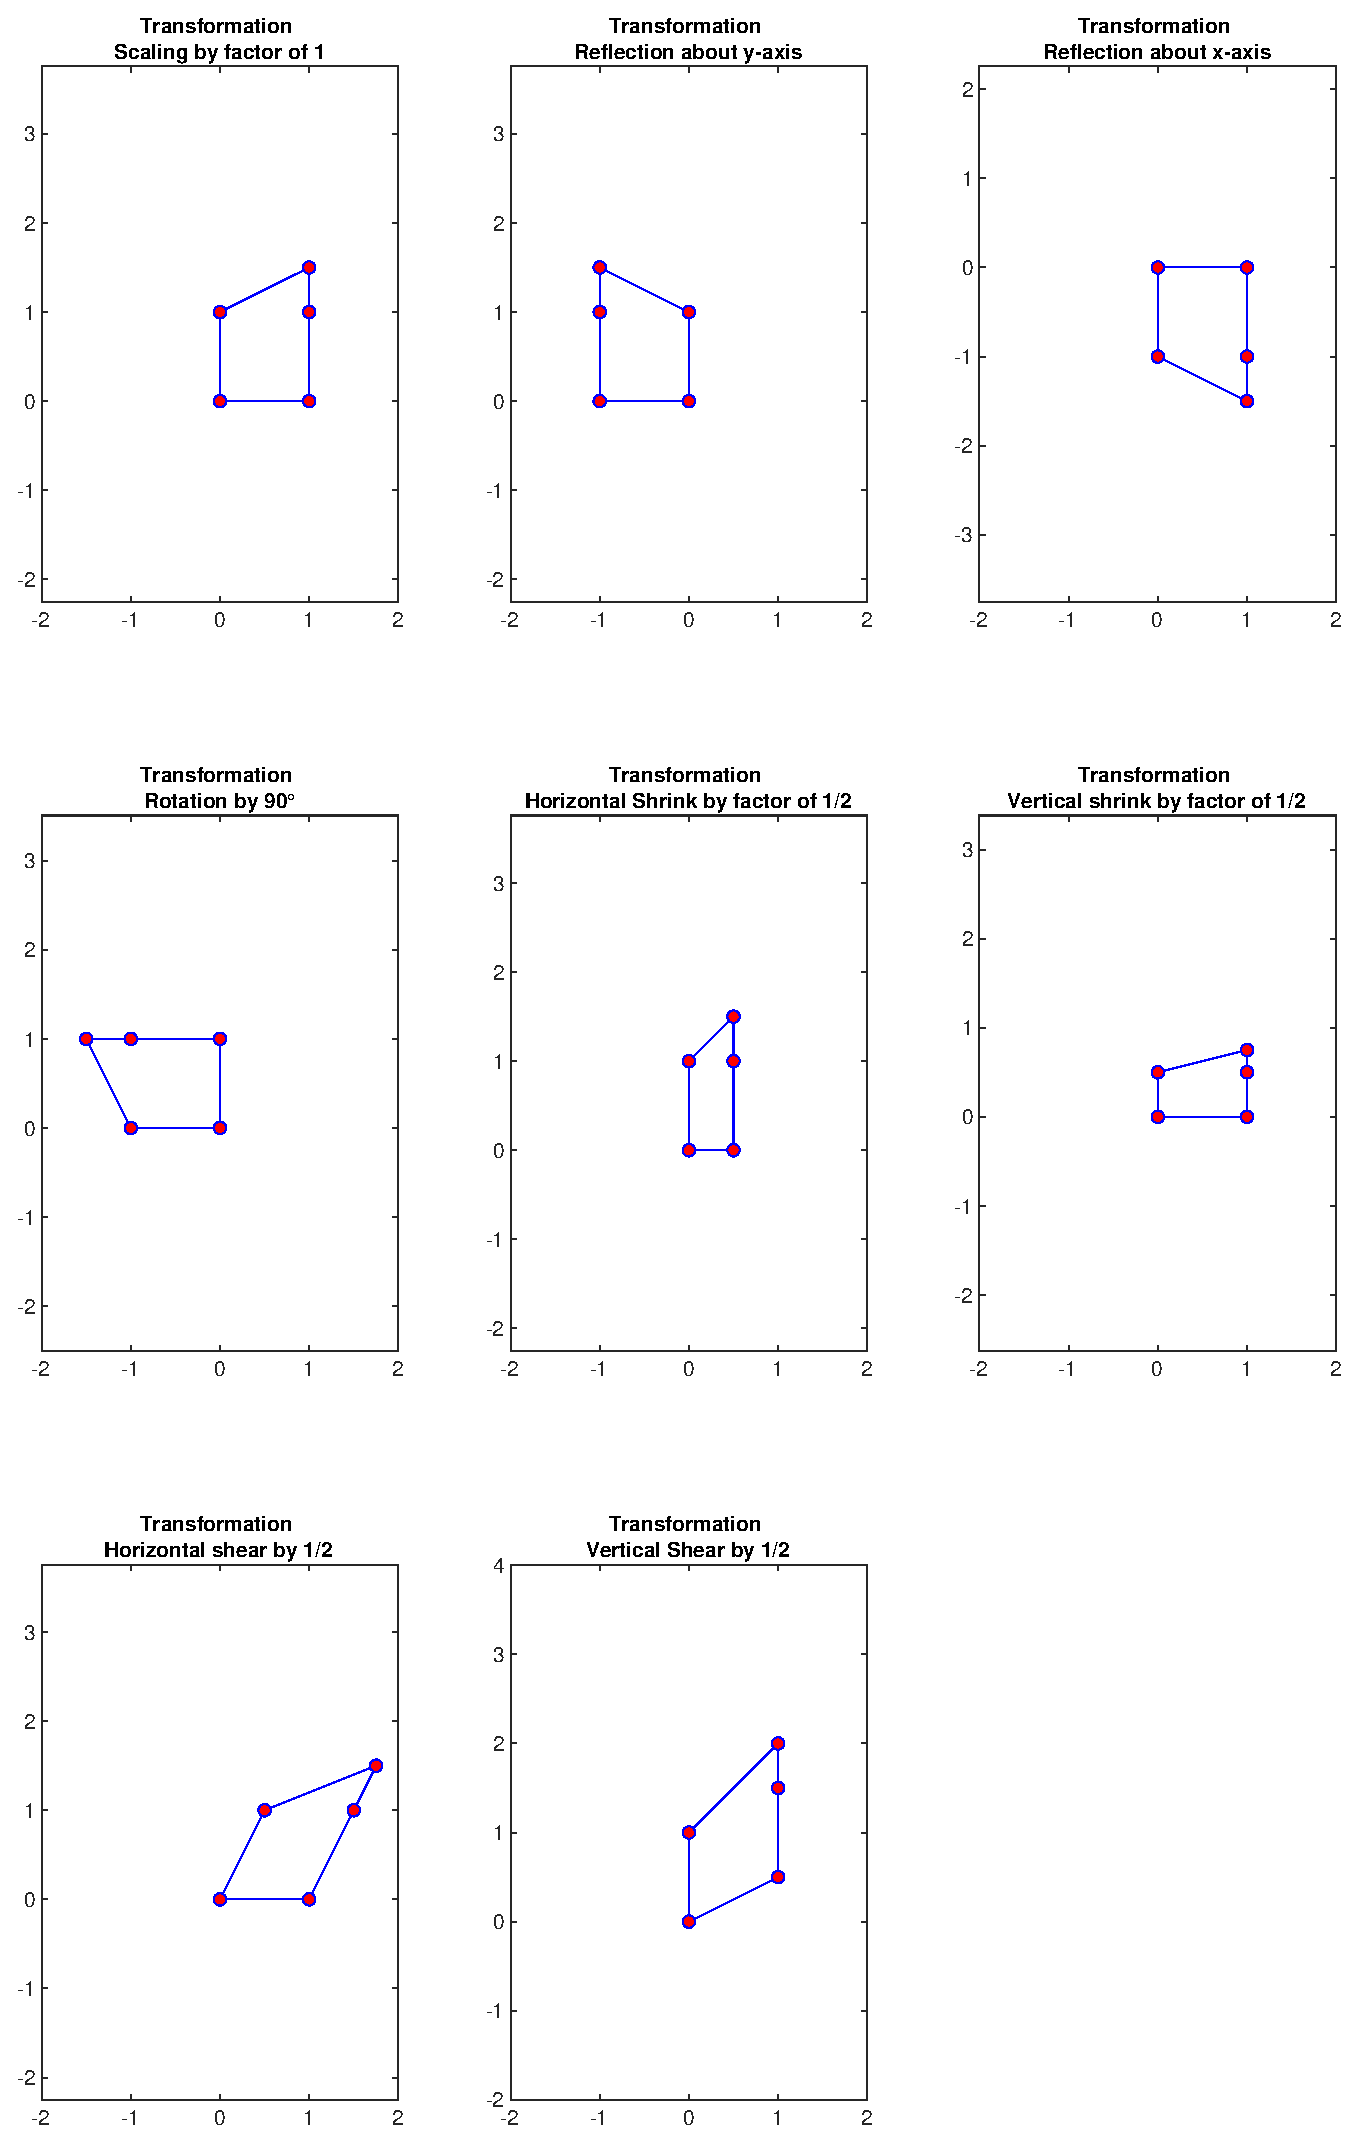
\includegraphics [width=4in]{transformations_02.eps}



\end{document}

